\documentclass[border=1pt]{standalone}
\usepackage[dvipsnames]{xcolor}
\usepackage{tikz}                       % Graphen und kommutative Diagramme
\usetikzlibrary{patterns}               % Um schraffierte Formen in der tikzpicture-Umgebung zu zeichnen.
\newcommand{\ul}[1]{\underline{\smash{#1}}}

\begin{document}
\centering
\resizebox{!}{2cm}
{
    \raisebox{-0.5\height}
    {
        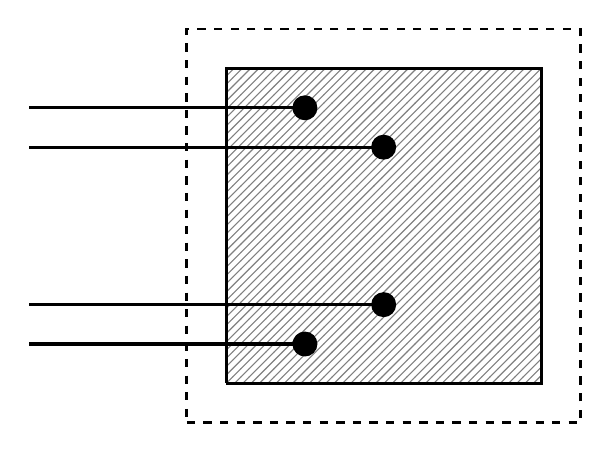
\begin{tikzpicture}[line width=1pt]
            % draw shaded slit box
            \filldraw[pattern=north east lines, pattern color=black!50] (0.5, 0.5) -- (4.5, 0.5) -- (4.5, 4.5) -- (0.5, 4.5) -- (0.5, 0.5);
            
            % draw outer lines
            \draw[dashed] (0, 0) -- (5, 0) -- (5, 5) -- (0, 5) -- (0, 0);
                
            % draw slits
            \draw[color=black, line width=1.2pt] (-2, 1.5) -- (2.5, 1.5);
            \filldraw (2.5, 1.5)   circle (4pt);
            \draw[color=black, line width=1.2pt] (-2, 1) -- (1.5, 1);
            \filldraw (1.5, 1)   circle (4pt);
            \draw[color=black, line width=1.2pt] (-2, 3.5) -- (2.5, 3.5);
            \filldraw (2.5, 3.5)   circle (4pt);
            \draw[color=black, line width=1.2pt] (-2, 4) -- (1.5, 4);
            \filldraw (1.5, 4)   circle (4pt);
        \end{tikzpicture}
    }
    \hspace{4cm}
%     \raisebox{-0.5\height}
%     {       
%         \begin{tikzpicture}[line width=1pt]
%             % draw shaded slit box
%             \filldraw[pattern=north east lines, pattern color=black!50] 
%             (100 : 2) -- (100: 4) arc [radius = 4, start angle = 100, delta angle =  160] 
%                       -- (260: 2) arc [radius = 2, start angle = 260, delta angle = -160] ;
%             
%             % draw inner and outer circles
%             \draw (50 : 1) -- ( 50 : 5) arc [radius = 5, start angle =  50, delta angle =  260] 
%                            -- (310 : 1) arc [radius = 1, start angle = 310, delta angle = -260] ;
% 
%             % draw slits
%             \draw[color=black, line width=1.2pt] (120 : 5) -- (120 : 3.33);
%             \filldraw (120 : 3.33)   circle (4pt);
%             \draw[color=black, line width=1.2pt] (140 : 5) -- (140 : 2.66);
%             \filldraw (140 : 2.66)   circle (4pt);
%             \draw[color=black, line width=1.2pt] (220 : 5) -- (220 : 2.66);
%             \filldraw (220 : 2.66)   circle (4pt);
%             \draw[color=black, line width=1.2pt] (240 : 5) -- (240 : 3.33);
%             \filldraw (240 : 3.33)   circle (4pt);
%         \end{tikzpicture}
%     }
%     \hspace{4cm}
    \raisebox{-0.5\height}
    {
        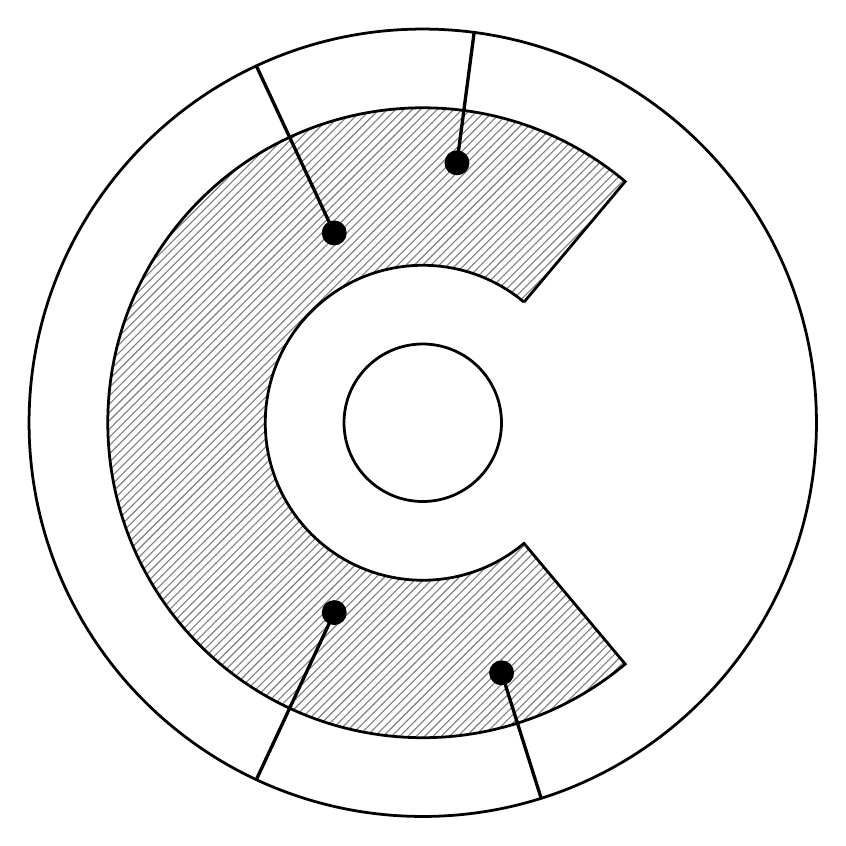
\begin{tikzpicture}[line width=1pt]
            % draw shaded slit box
            \filldraw[pattern=north east lines, pattern color=black!50] 
            (50 : 2) -- ( 50 : 4) arc [radius = 4, start angle =  50, delta angle =  260] 
                     -- (310 : 2) arc [radius = 2, start angle = 310, delta angle = -260] ;
            
            % draw inner and outer circles
            \draw[color=black] (0, 0) circle (1);
            \draw[color=black] (0, 0) circle (5);

            % draw slits
            \draw[color=black, line width=1.2pt] (82.5 : 5) -- (82.5 : 3.33);
            \filldraw (82.5 : 3.33)   circle (4pt);
            \draw[color=black, line width=1.2pt] (115 : 5) -- (115: 2.66);
            \filldraw (115 : 2.66)   circle (4pt);
            \draw[color=black, line width=1.2pt] (245 : 5) -- (245 : 2.66);
            \filldraw (245 : 2.66)   circle (4pt);
            \draw[color=black, line width=1.2pt] (287.5 : 5) -- (287.5 : 3.33);
            \filldraw (287.5 : 3.33)   circle (4pt);
        \end{tikzpicture}
    }
}
\end{document}
